\documentclass[12pt,dvipdfmx]{article}
\setlength{\oddsidemargin}{-1.3truecm}
\setlength{\evensidemargin}{-1.3truecm}
\setlength{\textwidth}{18.5truecm}
\setlength{\headsep}{1truecm}
\setlength{\topmargin}{-2truecm}
\setlength{\textheight}{23truecm}
\usepackage{graphicx}
\DeclareGraphicsExtensions{.pdf}
\DeclareGraphicsExtensions{.eps}
\graphicspath{{out/}{out/tex/}{out/tex/gpl/}{out/tex/svg/}{out/tex/dot/}}
%\graphicspath{{out/}{out/tex/}{out/pdf/}{out/eps/}{out/tex/gpl/}{out/tex/svg/}{out/pdf/dot/}{out/pdf/gpl/}{out/pdf/img/}{out/pdf/odg/}{out/pdf/svg/}{out/eps/dot/}{out/eps/gpl/}{out/eps/img/}{out/eps/odg/}{out/eps/svg/}}
\usepackage{listings}
\usepackage{fancybox}
\usepackage{hyperref}
\usepackage{color}

\lstset{language = python,
numbers = left,
numberstyle = {\tiny \emph},
numbersep = 10pt,
breaklines = true,
breakindent = 40pt,
frame = tlRB,
frameround = ffft,
framesep = 3pt,
rulesep = 1pt,
rulecolor = {\color{blue}},
rulesepcolor = {\color{blue}},
flexiblecolumns = true,
keepspaces = true,
basicstyle = \ttfamily\scriptsize,
identifierstyle = ,
commentstyle = ,
stringstyle = ,
showstringspaces = false,
tabsize = 4,
escapechar=\@,
}

\title{Incompressible Flow}
\author{田浦}
\date{}

\begin{document}
\maketitle

\section{やりたいこと}
2次元ハーゲン・ポアズイユ流を以下の領域でシミュレートしたい

\begin{center}
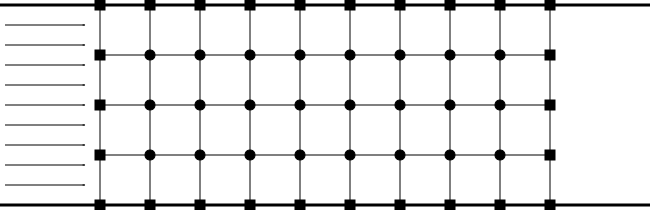
\includegraphics[width=0.6\textwidth]{out/pdf/svg/flow.pdf}
\end{center}

\section{方程式}

\begin{equation}
  \frac{\partial u}{\partial t}
  = - (u \cdot \nabla) u - \nabla p + c \Delta u
  \label{eq:navier}
\end{equation}
\begin{equation}
  \nabla \cdot u = 0
  \label{eq:cont}
\end{equation}

\section{解法}
非圧縮の方程式の普通の解き方.

右辺の$p$を求めるために式(\ref{eq:navier})の両辺の$\nabla \cdot$をとる.
\begin{equation}
\frac{\partial \nabla\cdot u}{\partial t}
  + \nabla \cdot (- (u \cdot \nabla) u - \nabla p + c \Delta u) h
\end{equation}

連続の式(\ref{eq:cont})より
$\nabla \cdot u = 0$なので
\begin{equation}
  0 = \nabla \cdot (- (u \cdot \nabla) u - \nabla p + c \Delta u)
\end{equation}
よって
\begin{equation}
  - \nabla \cdot (u \cdot \nabla) u - \Delta p + c \nabla \cdot \Delta u = 0
\end{equation}
さらに
\begin{equation}
\nabla \cdot \Delta u = \Delta (\nabla \cdot u) = 0
\end{equation}
なので,
\begin{equation}
  \Delta p = - \nabla \cdot (u \cdot \nabla) u
  \label{eq:poisson}
\end{equation}
よって, 1ステップの計算は,

\begin{enumerate}
\item 式(\ref{eq:poisson})を用いて$p$を求める.
  \begin{equation}
    \Delta p = - \nabla \cdot (u \cdot \nabla) u
    \label{eq:poisson}
  \end{equation}
\item 求まった$p$を用いて, $u(t+h)$を求める.
  \begin{equation}
    u(t + h) \approx u(t) + (- (u \cdot \nabla) u - \nabla p + c \Delta u) h
    \label{eq:step}
  \end{equation}
\end{enumerate}

\section{計算の方法$+$よくわからないこと}
一番単純に各格子点に$p$, $u$を割り当てて
(スタッガード格子とかは必要だとわかるまでとりあえずやらないで),
差分法で解こうと思っている.

その際に境界条件の与え方がよくわからない.

\begin{enumerate}
\item 圧力の式(\ref{eq:poisson})を解くときの境界条件は?

  どこぞには, ノイマン条件を課すみたいなことが書いてある.

  \begin{equation}
  \frac{\partial p}{\partial n} = 0 \label{eq:boundary_p}
  \end{equation}
  
\item $u$に関する境界条件は?

  \begin{equation}
    \mbox{上下の壁沿いについては}u = 0 \label{eq:eq:boundary_top_bottom}
  \end{equation}
  でよいなのだろう(多分).

  では左右の空いているところはどうしたら良い? (ここが一番良くわからない)

  とりあえずよくわからないながら,

  \begin{equation}
    \mbox{左(流入して来る所)については} u = (1, 0), \label{eq:boundary_left}
  \end{equation}
  \begin{equation}
    \mbox{右(流出して行く所)については}
    \frac{\partial u}{\partial n} = 0 \label{eq:boundary_right}
  \end{equation}
  という条件を課している. 後者の$n$は$x$軸方向のベクトル.
  最終的に得たい答えはポアズイユ流の,
  $u_x = (y - 1/2)^2$ みたいな答えなので, 明らかに違うのだが,
  と言って, まさかこれを境界条件というわけにも行かず,
  どうしたものかという感じ.
\end{enumerate}

ちなみに差分法で計算するときの表面的な問題として,
格子点の数を$m \times n$とすると,
式(\ref{eq:poisson})の右辺を作る時に微分を差分で計算する関係で,
右辺が計算できるのは, 内部の点($(m - 2) \times (n - 2)$)だけになる.
従って, 連立一次方程式を用いて求まる$p$も内部の点だけとなる
(ノイマン条件を課しているので,
外周の点は内部の点と同じとして計算する.
つまり, $p[0,j] = p[1,j]$, $p[m-1,j] = p[m-2,j]$, $p[i,0] = p[i,1]$, $p[i,n-1] = p[i,n-2]$).

そうやって求まった($m \times n$点の)$p$を用いて
式(\ref{eq:step})の右辺を計算するときも, やはり微分を差分で作る関係で,
右辺が計算できるのは内部の点だけとなる.
そのため外周の点に対しては$u(t + h)$の値が(少なくとも素直には)求まらない.
壁沿いについては物理的に直感にあう境界条件(式\ref{eq:boundary_top_bottom})があるわけだが, 左右の空いているところはさてどうするのが良いのだろう.

コードを添付します.
matplotlibが必要です.
python3 で走らせてくれれば勝手にアニメーションが
始まるはずです.

やってみると最初のうち中なか変化がないけど,
よく見ると徐々に色が変わってきます.
そしてそのうちに破綻した感じにぐちゃぐちゃになります.

何が悪いのか.

\begin{itemize}
\item 境界条件が悪い
\item dtの値が大きすぎる
\item オイラー法が荒すぎる
\item 空間微分が荒すぎる
\item ポアソン方程式の行列の係数のところでバグを入れている
\item \ldots 
\end{itemize}
など色々あるとおもうのですが.
あまりこれ以上一人で悶々と悩みたくないので,
頭の整理を兼ねてこんな文章を書いてみたというわけです.

\section{付録: コード}
\lstinputlisting{../incompressible.py}

\end{document}
